\section{Motivation}
\label{sec:motive}

\begin{table}
\begin{center}
\small
\begin{tabular}{lrrr}
   & \multicolumn{2}{c}{\textbf{Latency (µs)}} & \textbf{Throughput} \\
  \textbf{Isolation method} & Median & 99\% & \textbf{(invocations/sec)} \\
\midrule
Process-based & 8.7 & 27.3 & .29 million \\
Language-based & 1.2 & 2.0 & 5.4 million \\
\end{tabular}
\caption{Performance of isolation methods}
\label{tab:isolation_methods}
\end{center}
\end{table}

Our decision to use language-based isolation is based on two experimental
findings:  First, process-level isolation is too slow for
microsecond-scale remote functions. Second, high-precision timers on commodity
CPUs allow preemption at microsecond scale.  We conducted these experiments
on an Intel Xeon E5-2683 v4 server (16 cores, 2.1~GHz) running
Linux 4.13.0; we discuss the results below.

\subsection{Process-level isolation is too slow}
We run the following experiment to evaluate the overhead of different isolation
techniques. We use 14 \emph{worker} CPU cores to run microservices. Another core runs
runs a \emph{host} process that initiates microservice execution on the workers.
The host schedules up to 14 microservices at a time (i.e., one
per worker core), choosing from a pool of 5,000 microservices. It uses one of two
methods to run microservices:

\begin{enumerate}
\item \textbf{Process-based isolation:} Each microservice is a separate process.
At any time, most microservice processes are blocked on an IPC
call. The host runs a microservice by waking up its process using a UDP datagram.
\solb{Sources say other IPC methods could be a bit faster; should we test?}
\ak{Would be a nice addition if there's time.}
\item \textbf{Language-based isolation:} Each worker core runs a single-threaded
\emph{worker process} that is used to run different microservices, one at a time.
In this approach, shown in Figure~\ref{fig:sysdesign}, a worker process runs a
microservice by calling its registered
function; we assume that the microservice function can be isolated from the
worker process with language-based isolation techniques that we discuss in
Section~\ref{sec:isolation}. The host schedules microservices on worker processes by
sending them
requests on a shared memory queue. Worker processes poll this queue to receive
new requests.
\end{enumerate}

\begin{figure}
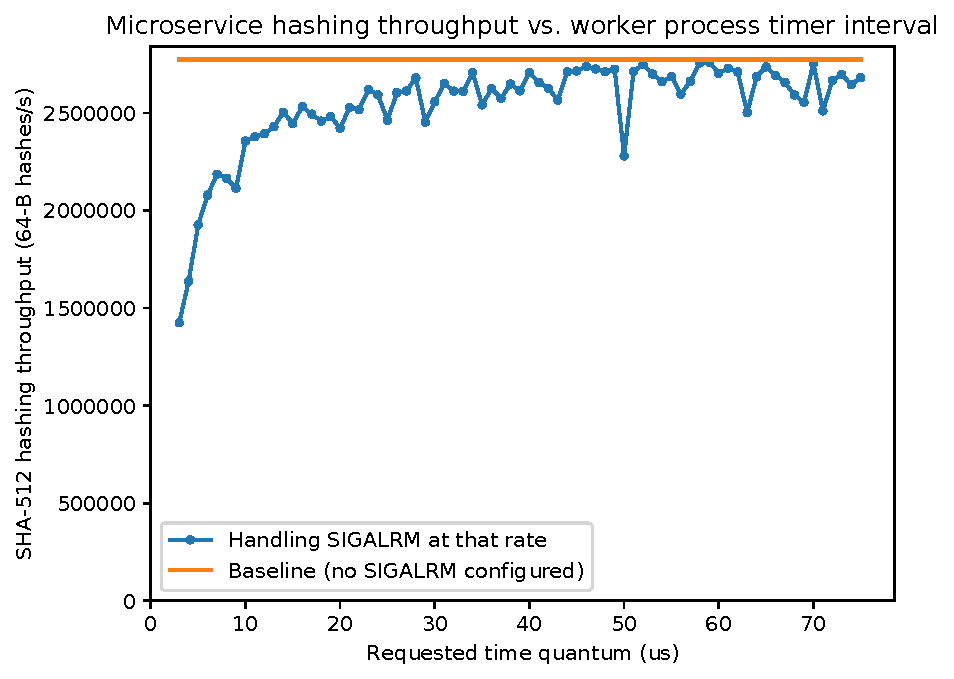
\includegraphics[width=\columnwidth]{figs/system}
\caption{Design of the language-based isolation approach.  The host process forwards
requests over a shared-memory queue to a number of worker processes, each of which
runs one user-supplied microservice at a time.}
\label{fig:sysdesign}
\end{figure}

Table~\ref{tab:isolation_methods} shows the latency and throughput achieved
by the two methods. For latency, we measure the time between when the host
process dispatches a request to a microservice and when the microservice begins
useful work on a worker core. We find that the process-based isolation approach
takes \us{9} and achieves only 300,000 microservice invocations per
second. In contrast, language-based isolation achieves \us{1.2} (with a tail
of just \us{2.0}) and over 5 million invocations per second.\footnote{We also
observe that, with trivial microservices, there is a difference in memory
footprint: for 5,000 resident microservices, the system memory usage rises by about
2 GiB for the process-based approach, versus just 1.3 for the language-based one.  Of
course, these numbers will substantially rise for larger programs, but we expect the
gap to widen as various registered microservices include the same libraries.}
\ak{Not sure if we need this footnote.}

A \us{9} delay in microservice invocation is already a substantial fraction of
Azure's \us{20} RPC latency, a fraction that will only increase with
improvements in network latency. We therefore conclude that even in the average case,
process-based isolation is too slow for microsecond-scale scheduling; furthermore,
invocation throughput is also limited by IPC overhead.

\subsection{Intra-process preemption is fast}
With language-based isolation, we run user-provided microservice functions
directly in worker processes. To prevent rogue functions from endlessly blocking
other microservices, we must premept or terminate functions that run for too
long (e.g., longer than \us{100}).  This preemption interval is orders of
magnitude faster than Linux's default 4ms time quantum.

Fortunately, we found that high-precision event timers (HPETs) on modern CPUs
are sufficient for this task. We measure the granularity and reliability of
these timers as follows: We run one thread that requests a periodic timer with a
configurable interval of $T$~\textmu{}s and installs an associated signal handler.
Ideally, this handler would always be called exactly $T$~\textmu{}s after its last
invocation; we measure the deviation from $T$ over 256 iterations.
We find that the variance
is smaller than 0.3~\textmu{}s for $T \ge 3$~\textmu{}s. This shows that
intra-process preemption is fast and reliable enough for our needs.
